% NB: use pdflatex to compile NOT pdftex.  Also make sure youngtab is
% there...

% converting eps graphics to pdf with ps2pdf generates way too much
% whitespace in the resulting pdf, so crop with pdfcrop
% cf. http://www.cora.nwra.com/~stockwel/rgspages/pdftips/pdftips.shtml




\documentclass[10pt,dvipsnames]{beamer}
\usetheme[color/block=transparent]{metropolis}

\usepackage[absolute,overlay]{textpos}
\usepackage{booktabs}
\usepackage[utf8]{inputenc}

\usepackage{tikz}
\usetikzlibrary{arrows.meta}


\usepackage[scale=2]{ccicons}

\usepackage[official]{eurosym}


%use this to add space between rows
\newcommand{\ra}[1]{\renewcommand{\arraystretch}{#1}}


\newcommand{\R}{\mathbb{R}}



\setbeamerfont{alerted text}{series=\bfseries}
\setbeamercolor{alerted text}{fg=Mahogany}
\setbeamercolor{background canvas}{bg=white}


\def\l{\lambda}
\def\m{\mu}
\def\d{\partial}
\def\cL{\mathcal{L}}
\def\co2{CO${}_2$}
\def\bra#1{\left\langle #1\right|}
\def\ket#1{\left| #1\right\rangle}
\newcommand{\braket}[2]{\langle #1 | #2 \rangle}
\newcommand{\norm}[1]{\left\| #1 \right\|}
\def\corr#1{\Big\langle #1 \Big\rangle}
\def\corrs#1{\langle #1 \rangle}



% for sources http://tex.stackexchange.com/questions/48473/best-way-to-give-sources-of-images-used-in-a-beamer-presentation

\setbeamercolor{framesource}{fg=gray}
\setbeamerfont{framesource}{size=\tiny}


\newcommand{\source}[1]{\begin{textblock*}{4cm}(8.0cm,8.0cm)
    \begin{beamercolorbox}[ht=0.5cm,right]{framesource}
        \usebeamerfont{framesource}\usebeamercolor[fg]{framesource} Source: {#1}
    \end{beamercolorbox}
\end{textblock*}}

\usepackage{hyperref}

\usepackage{tikz}


\usepackage{circuitikz}

%\usepackage[pdftex]{graphicx}


\graphicspath{{graphics/}}

\DeclareGraphicsExtensions{.pdf,.jpeg,.png,.jpg,.gif}



\def\goat#1{{\scriptsize\color{green}{[#1]}}}



\let\olditem\item
\renewcommand{\item}{%
\olditem\vspace{5pt}}

\title{Energy System Modelling\\ Summer Semester 2019, Lecture 4}
%\subtitle{---}
\author{
  {\bf Dr. Tom Brown}, \href{mailto:tom.brown@kit.edu}{tom.brown@kit.edu}, \url{https://nworbmot.org/}\\
  \emph{Karlsruhe Institute of Technology (KIT), Institute for Automation and Applied Informatics (IAI)}
}

\date{\vspace{.3cm}7th June 2019}


\titlegraphic{%
  \vspace{6cm}
  \hspace{6.7cm}
    \includegraphics[trim=0 0cm 0 0cm,height=1.8cm,clip=true]{kit.png}
}

\begin{document}

\maketitle


\begin{frame}

  \frametitle{Table of Contents}
  \setbeamertemplate{section in toc}[sections numbered]
  \tableofcontents[hideallsubsections]
\end{frame}


\section{Revising Ohm's Law}

\begin{frame}
  \frametitle{Ohm's Law}

  \alert{Ohm's Law}: The potential difference (voltage) $V_1 - V_2$ across an ideal conductor is proportional to the current through it $I$. The constant of proportionality is called the \alert{resistance}, $R$. Ohm's Law is thus:
  \begin{equation*}
     V_1 - V_2 = I\,R
  \end{equation*}

  \centering
  \includegraphics[width=8cm]{ohm_law.png}


\end{frame}

\begin{frame}
  \frametitle{Analogy DC circuits to linear power flow}

  The equations for DC circuits and linear power flow in AC circuits are analogous:
  \begin{equation*}
    I = \frac{V_i - V_j}{R} \hspace{.55cm} \leftrightarrow \hspace{.55cm} f_\ell =  \frac{\theta_i - \theta_j}{x_\ell}
  \end{equation*}

  if we make the following identification:
    \ra{1.05}
  \begin{table}[!t]
    \begin{tabular}{p{4cm}p{0.5cm}p{4cm}}
      \toprule
      Current flow $I$ & $\leftrightarrow$  &  Active power flow $f_\ell$ \\
      Potential/voltage $V_i$ & $\leftrightarrow$  &  Voltage angle $\theta_i$ \\
      Resistance $R$ & $\leftrightarrow$  &  Reactance $X$ \\
      \bottomrule
    \end{tabular}
  \end{table}

  The simplifications that lead to the linear power flow were explained in the previous lecture.

\end{frame}


\begin{frame}
  \frametitle{Kirchhoff's Current Law (KCL)}

  KCL inforces energy conservation at each vertex (the power imbalance
  equals what goes out minus what comes in).

  \vspace{.3cm}

  \begin{columns}
    \column[c]{.5\textwidth}


    \centering

  %https://tex.stackexchange.com/questions/270543/draw-a-graph-in-latex-with-tikz
  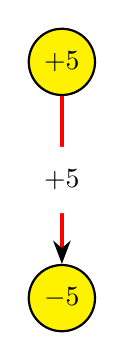
\begin{tikzpicture}
    \begin{scope}[every node/.style={circle,thick,draw,fill=yellow}]
      \node (1) at (0,3) {$+5$};
      \node (2) at (0,0) {$-5$};
    \end{scope}

    \begin{scope}[>={Stealth[black]},
        every node/.style={fill=white,circle},
        every edge/.style={draw=red,very thick}]
      \path [->] (1) edge node {$+5$} (2);
    \end{scope}
  \end{tikzpicture}

    \column[c]{.5\textwidth}


    \centering

  %https://tex.stackexchange.com/questions/270543/draw-a-graph-in-latex-with-tikz
  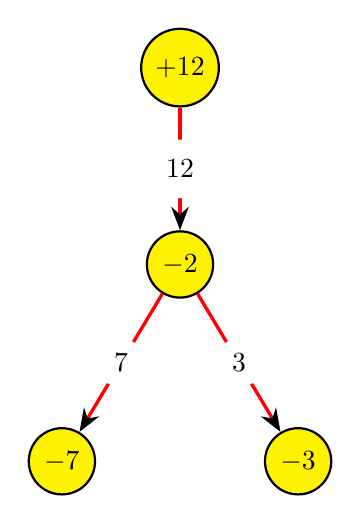
\begin{tikzpicture}
    \begin{scope}[every node/.style={circle,thick,draw,fill=yellow}]
      \node (1) at (1.5,5) {$+12$};
      \node (2) at (1.5,2.5) {$-2$};
      \node (3) at (0,0) {$-7$};
      \node (4) at (3,0) {$-3$};
    \end{scope}

    \begin{scope}[>={Stealth[black]},
        every node/.style={fill=white,circle},
        every edge/.style={draw=red,very thick}]
      \path [->] (1) edge node {$12$} (2);
      \path [->] (2) edge node {$7$} (3);
      \path [->] (2) edge node {$3$} (4);
    \end{scope}
  \end{tikzpicture}


  \end{columns}

\end{frame}





\begin{frame}
  \frametitle{Kirchhoff's Voltage Law (KVL)}

  KCL isn't enough to determine the flow as soon as there are \alert{closed cycles} in the network.
   For this we need Ohm's law in combination with KVL: voltage
  differences around each cycle add up to zero.

  \vspace{.3cm}

  \begin{columns}
    \column[c]{.5\textwidth}


    \centering

  %https://tex.stackexchange.com/questions/270543/draw-a-graph-in-latex-with-tikz
  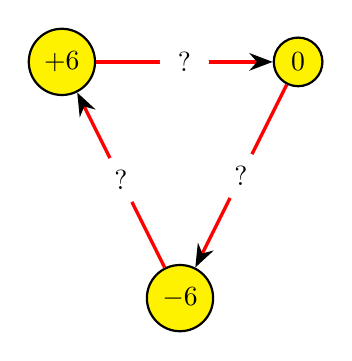
\begin{tikzpicture}
    \begin{scope}[every node/.style={circle,thick,draw,fill=yellow}]
      \node (1) at (0,3) {$+6$};
      \node (2) at (3,3) {$0$};
      \node (3) at (1.5,0) {$-6$};
    \end{scope}

    \begin{scope}[>={Stealth[black]},
        every node/.style={fill=white,circle},
        every edge/.style={draw=red,very thick}]
      \path [->] (1) edge node {$?$} (2);
      \path [->] (2) edge node {$?$} (3);
      \path [->] (3) edge node {$?$} (1);
    \end{scope}
  \end{tikzpicture}


      \column[c]{.5\textwidth}


      For equal reactances for each edge:


  \vspace{.3cm}

    \centering
  %https://tex.stackexchange.com/questions/270543/draw-a-graph-in-latex-with-tikz
  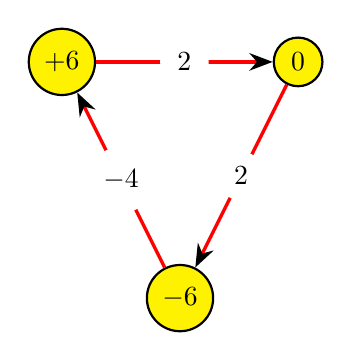
\begin{tikzpicture}
    \begin{scope}[every node/.style={circle,thick,draw,fill=yellow}]
      \node (1) at (0,3) {$+6$};
      \node (2) at (3,3) {$0$};
      \node (3) at (1.5,0) {$-6$};
    \end{scope}

    \begin{scope}[>={Stealth[black]},
        every node/.style={fill=white,circle},
        every edge/.style={draw=red,very thick}]
      \path [->] (1) edge node {$2$} (2);
      \path [->] (2) edge node {$2$} (3);
      \path [->] (3) edge node {$-4$} (1);
    \end{scope}
  \end{tikzpicture}

  \raggedright
  NB: For directed graph, sign determines direction of flow.

  \end{columns}
\end{frame}



\section{Computing the Linear Power Flow}

\begin{frame}
  \frametitle{Framing the load flow problem}

  Suppose we have $N$ nodes labelled by $i$, and $L$ edges labelled by
  $\ell$ forming a directed graph $G$.

  Suppose at each node we have a \alert{power imbalance} $p_i$ ($p_i >
  0$ means its generating more than it consumes and $p_i < 0$ means it
  is consuming more than it).

  Since we cannot create or destroy energy (and we're ignoring losses):
  \begin{equation*}
    \sum_i p_i = 0
  \end{equation*}

  \alert{Question}: How do the flows $f_\ell$ in the network relate to the nodal power
  imbalances?

  \alert{Answer}: According to the impedances (generalisation of
  resistance for oscillating voltage/current) and the corresponding
  voltages.

\end{frame}



\begin{frame}
  \frametitle{Kirchhoff's Current Law (KCL)}

  KCL says (in this linear setting) that the nodal power imbalance at
  node $i$ is equal to the sum of direct flows arriving at the
  node. This can be expressed compactly with the incidence matrix

  \begin{equation*}
    p_i = \sum_\ell K_{i\ell} f_\ell \hspace{2cm} \forall i
  \end{equation*}


\end{frame}


\begin{frame}
  \frametitle{Kirchhoff's Voltage Law (KVL)}

  KVL says that the sum of voltage differences across edges for any
  closed cycle must add up to zero.

  If the voltage at any node is given by $\theta_i$ (this is infact
  the voltage \alert{angle} - more next week) then the voltage difference across edge $\ell$ is
  \begin{equation*}
    \sum_i K_{i\ell} \theta_i
  \end{equation*}

  And Kirchhoff's law can be expressed using the cycle matrix encoding of independent cycles
  \begin{equation*}
    \sum_\ell C_{\ell c} \sum_i K_{i\ell} \theta_i = 0 \hspace{2cm} \forall c
  \end{equation*}

  [Automatic, since we already said KC = 0.]


\end{frame}



\begin{frame}
  \frametitle{Kirchhoff's Voltage Law (KVL)}

  If we express the flow on each line in terms of the voltage angle (a
  relative of $V = IR$) then for a line $\ell$ with reactance $x_\ell$
  \begin{equation*}
    f_\ell = \frac{\theta_i - \theta_j}{x_\ell} = \frac{1}{x_\ell}\sum_{i} K_{i\ell} \theta_i
  \end{equation*}

  KVL now becomes
  \begin{equation*}
    \sum_\ell C_{\ell c} x_\ell f_\ell = 0 \hspace{2cm} \forall c
  \end{equation*}

\end{frame}



\begin{frame}
  \frametitle{Solving the equations}

  If we combine
    \begin{equation*}
    f_\ell  = \frac{1}{x_\ell}\sum_{i} K_{i\ell} \theta_i
  \end{equation*}
    with Kirchhoff's Current Law we get
    \begin{equation*}
    p_i = \sum_{\ell} K_{i\ell}f_\ell =   \sum_{\ell} K_{i\ell} \frac{1}{x_\ell}\sum_{j} K_{j\ell} \theta_j
    \end{equation*}
    This is a \alert{weighted Laplacian}. If we write $B_{k\ell}$ for the diagonal matrix with $B_{\ell\ell} = \frac{1}{x_\ell}$ then
    \begin{equation*}
      L = KBK^t
    \end{equation*}
    and we get a \alert{discrete Poisson equation} for the $\theta_i$ sourced by the $p_i$
    \begin{equation*}
      p_i = \sum_{j} L_{ij} \theta_j
    \end{equation*}
    We can solve this for the $\theta_i$ and thus find the flows.

\end{frame}


\begin{frame}
  \frametitle{Solving the equations}

  Given $p_i$ at every node, we want to find the flows $f_\ell$. We
  have the equations
    \begin{align*}
      p_i & = \sum_{j} L_{ij} \theta_j \\
     f_\ell  & = \frac{1}{x_\ell}\sum_{i} K_{i\ell} \theta_i
    \end{align*}

    Basic idea: invert $L$ to get $\theta_i$ in terms of $p_i$
    \begin{equation*}
      \theta_i  = \sum_{k} (L^{-1})_{ik} p_k
    \end{equation*}
    then insert to get the flows as a linear function of the power injections $p_i$
    \begin{equation*}
    f_\ell   = \frac{1}{x_\ell}\sum_{i,k} K_{i\ell}  (L^{-1})_{ik} p_k = \sum_k \textrm{PTDF}_{\ell k} p_k
    \end{equation*}
    called the \alert{Power Transfer Distribution Factors} (PTDF).

\end{frame}


\begin{frame}
  \frametitle{Inverting Laplacian $L$}

  There is one small catch: $L$ is \alert{not invertible} since we saw last
  time it has (for a connected network) one zero eigenvalue, with
  eigenvector $(1,1, \dots 1)$, since by construction $\sum_j L_{ij} =
  0$.

  This is related to a gauge freedom to add a constant to all voltage angles
  \begin{equation*}
    \theta_i \to \theta_i + c
  \end{equation*}
  (corresponding to the zero eigenvector of $L$) which does not affect physical quantities:
    \begin{align*}
      p_i & = \sum_{j} L_{ij} (\theta_j+ c) = \sum_{j} L_{ij} (\theta_j)  \\
     f_\ell  & = \frac{1}{x_\ell}\sum_{i} K_{i\ell}( \theta_i  + c) = \frac{1}{x_\ell}\sum_{i} K_{i\ell}( \theta_i )
    \end{align*}

    Typically we choose a \alert{slack} or \alert{reference bus} such that  $\theta_1 = 0$.


\end{frame}

\begin{frame}
  \frametitle{Inverting Laplacian $L$}

  Two solutions:

  1. Since $\theta_1 = 0$ and $p_1$ is not independent of the other
  power injections ($\sum_{i=1}^N p_i = 0$ implies $p_1 = -
  \sum_{i=2}^N p_i$), we can ignore these elements and invert
  the lower-right $(N-1) \times (N-1)$ part of $L$ (which doesn't have zero eigenvalues) to find the
  remaining $\{\theta_i\}_{i=2,\dots N}$ in terms of the
  $\{p_i\}_{i=2,\dots N}$.

  2. Use the Moore-Penrose pseudo-inverse.

  Write $L$ in terms of its basis of orthonormal eigenvectors $e^n_i$ ($\sum_j L_{ij} e^n_j = \l_n e^n_i$, $\sum_i e^n_i e^n_i = 1$ and  $\sum_i e^n_i e^m_i = 0$ if $n \neq m$):
  \begin{equation*}
    L_{ij} = \sum_n \l_n e^n_i e^n_j
  \end{equation*}
  then the Moore-Penrose pseudo-inverse is:
  \begin{equation*}
    L^\dagger_{ij} = \sum_{n | \l_n \neq 0} \frac{1}{\l_n} e^n_i e^n_j
  \end{equation*}
\end{frame}

\begin{frame}
  \frametitle{4-node example}

  \begin{columns}
\column[c]{.5\textwidth}
\begin{equation*}
\mathbf{K}_{i \ell}=\left(\begin{matrix}
1 & 0 & 0 & 0\\
-1 & 1 & 1 & 0\\
0 & -1 & 0 & 1\\
0 & 0 & -1 & -1
\end{matrix}\right)
\end{equation*}
\begin{equation*}
\mathbf{L}_{ij}=\left(\begin{matrix}
1 & -1 & 0 & 0\\
-1 & 3 & -1 & -1\\
0 & -1 & 2 & -1\\
0 & -1 & -1 & 2
\end{matrix}\right)
\end{equation*}
\begin{equation*}
\mathbf{PTDF}_{\ell i}=\left(\begin{matrix}
0 & -1 & -1 & -1\\
0 & 0 & -2/3 & -1/3\\
0 & 0 & -1/3 & -2/3\\
0 & 0 & 1/3 & -1/3
\end{matrix}\right)
\end{equation*}

\column[c]{.5\textwidth}
\includegraphics[scale=0.12]{graph19.png}
\end{columns}


\end{frame}



\begin{frame}
  \frametitle{PTDF as sensitivity}

  Can also `experimentally' determine the Power Transfer Distribution
  Factors (PTDF) by choosing a slack bus (in this case bus 1).

  Each column (labelled by $i$) is then the resulting line flows if we have
  a simple power transfer from bus $i$ to the slack $p_i = 1$ and $p_1
  = -1$.

  \begin{columns}
\column[c]{.5\textwidth}
\begin{equation*}
\mathbf{PTDF}_{\ell i}=\left(\begin{matrix}
0 & -1 & -1 & -1\\
0 & 0 & -2/3 & -1/3\\
0 & 0 & -1/3 & -2/3\\
0 & 0 & 1/3 & -1/3
\end{matrix}\right)
\end{equation*}

\column[c]{.5\textwidth}
\includegraphics[scale=0.12]{graph19.png}
\end{columns}


\end{frame}
\section{Consequences of limiting power transfers}



\begin{frame}
  \frametitle{Line loading limits}

  You cannot pass infinite current through a transmission line.

  As it warms, it sags, then it will become damaged and/or hit a
  building/tree and cause a short-circuit. For this reasons there are
  always \alert{thermal limits} on current transfer. There may also be
  limits on the amount of power or current based on concerns about
  \alert{voltage stability} or \alert{general stability}.

  Typically each line has a well-defined \alert{line loading limit} on the
  amount of current or power that can flow through it:
  \begin{equation*}
    | f_{\ell } | \leq F_\ell
  \end{equation*}
  where here $F_\ell$ is the maximum power capacity of the transmission lines.

  These limits prevent the transfer of renewable energy or other power sources.

\end{frame}




\begin{frame}
  \frametitle{Adjusting generator dispatch to avoid overloading}

  To avoid overloading the power lines, we must adjust our generator
  output (or the demand) so that the power imbalances do not overload
  the network.

  We will now generalise and adjust our notation.

  From lecture 2 we had for a single node:
  \begin{equation*}
    - p_t = m_t -b_t + c_t = d_t - Ww_t - Ss_t -b_t + c_t = 0
  \end{equation*}
  where $p_t$ was the nodal power balance, $m_t$ was the mismatch
  (load $d_t$ minus wind $Ww_t$ and solar $Ss_t$), $b_t$ was the
  backup power and $c_t$ was curtailment.

  We generalised this to multiple nodes labelled by $i$
  \begin{equation*}
    - p_{i,t} = m_{i,t} -b_{i,t} + c_{i,t} = d_{i,t} - W_iw_{i,t} - S_is_{i,t} -b_{i,t} + c_{i,t}
  \end{equation*}
  where now we don't enforce $p_{i,t} = 0$ but $\sum_{i} p_{i,t} = 0$ for
  all $t$.

\end{frame}


\begin{frame}
  \frametitle{Adjusting generator dispatch to avoid overloading} Now
  we write the dispatch of all generators at node $i$ (wind, solar,
  backup) labelled by technology $s$ as $g_{i,s,t}$ ($i$ labels node, $s$ technology and $t$ time) so that we have a relation between load $d_{i,t}$, generation $g_{i,s,t}$ and network flows $f_{\ell,t}$
  \begin{equation*}
    p_{i,t} = \sum_{s} g_{i,s,t} - d_{i,t} = \sum_{\ell} K_{i\ell} f_{\ell,t}
  \end{equation*}
  Where $s$ runs over the wind, solar and backup capacity generators
  (e.g. hydro or natural gas) at the node.

  A dispatchable generator's $g_{i,s,t}$ output can be controlled
  within the limits of its power capacity $G_{i,s}$
  \begin{equation*}
      0 \leq g_{i,s,t} \leq  G_{i,s}
  \end{equation*}
\end{frame}



\begin{frame}
  \frametitle{Variable generation constraints}

  For a renewable generator we have time series of availability $0\leq G_{i,s,t}\leq 1$ (the $s_t$ and $w_t$ before; $W$ and $S$ are the capacity $G_{i,s}$):
    \begin{equation*}
      0 \leq g_{i,s,t} \leq G_{i,s,t} G_{i,s} \leq  G_{i,s}
    \end{equation*}
    Curtailment corresponds to the case where $g_{i,s,t} < G_{i,s,t} G_{i,s}$:

  \begin{tikzpicture}
\node[anchor=south west,inner sep=0] (image) at (0,0) {\includegraphics[width=11cm]{scigrid-curtailment}};
\draw (3,2.7) node{$g_{i,s,t}$};
\draw (3,3.7) node{$G_{i,s,t}G_{i,s}$};
\draw (3,4.7) node{$G_{i,s}$};
  \end{tikzpicture}

\end{frame}

\begin{frame}
  \frametitle{Germany curtailment example}

  See \url{https://pypsa.org/examples/scigrid-lopf-then-pf.html}.

\end{frame}


\begin{frame}
  \frametitle{European transmission versus backup energy}

  Consider backup energy in a simplified European grid:

  \centering
  \includegraphics[trim=0 4cm 0 4cm,width=10cm,clip=true]{europe_map}

\end{frame}



\begin{frame}
  \frametitle{DE versus EU backup energy from last time}

  Germany needed backup generation for 31\% of total load:

  \centering
  \includegraphics[width=7cm]{mismatch-duration-DE}


  Europe needed Backup generation for only 24\% of the total load:

  \centering
  \includegraphics[width=7cm]{mismatch-duration-EU}

\end{frame}


\begin{frame}
  \frametitle{European transmission versus backup energy}

  \href{http://www.sciencedirect.com/science/article/pii/S0960148113005351}{Transmission needs across a fully renewable European power system} by Rodriguez, Becker, Andresen, Heide, Greiner, Renewable Energy, 2014

  \centering
  \includegraphics[width=10cm]{sarah_balancing.png}


\end{frame}

\section{Principles of electricity storage}


\begin{frame}
  \frametitle{Basic idea of storage}

  Networks were used to shift power imbalances between different
  places, i.e. in \alert{space}. Electricity storage can shift power in \alert{time}.

  \vspace{0.5cm}

  \begin{tikzpicture}
\node[anchor=south west,inner sep=0] (image) at (0,0) {\includegraphics[width=11cm]{mismatch-2011-07-01-2011-07-07}};
\draw[red,line width=5,->] (4,3) -- (4,4) -- (6.5,4) -- (6.5,2.5);
  \end{tikzpicture}

\end{frame}

\begin{frame}
  \frametitle{Storage consistency}

  Storage units, such as batteries or hydrogen storage, can both
  dispatch power within a certain capacity:
  \begin{equation*}
    0 \leq g_{i,s,t,\textrm{dispatch}} \leq G_{i,s,\textrm{dispatch}}
  \end{equation*}
  and consume power to store energy:
  \begin{equation*}
    0 \leq g_{i,s,t,\textrm{store}} \leq G_{i,s,\textrm{store}}
  \end{equation*}

  The total power can then be written:
  \begin{equation*}
    g_{i,s,t} = g_{i,s,t,\textrm{dispatch}}  - g_{i,s,t,\textrm{store}}
  \end{equation*}

  There is also a limit on the total energy $e_{i,s,t}$ at each time
  \begin{equation*}
    0 \leq e_{i,s,t} = e_{i,s,0} -\sum_{t'=1}^{t} g_{i,s,t'} \leq E_{i,s}
  \end{equation*}
  where $E_{i,s}$ is the energy capacity (in MWh). Or in iterative form
  \begin{align*}
    0 \leq e_{i,s,t} = e_{i,s,t-1} + g_{i,s,t,\textrm{store}} -  g_{i,s,t,\textrm{dispatch}} \leq E_{i,s}
  \end{align*}

\end{frame}

\begin{frame}
  \frametitle{Continuous example}

  Consider a single node with a constant demand
  \begin{equation*}
    d(t) = D
  \end{equation*}
  and a renewable wind generator with a capacity $G = 2D$ and an
  availability time series
  \begin{equation*}
    G(t) = \frac{1}{2} \left(1 + \sin\left(\frac{2\pi}{T} t\right)\right)
  \end{equation*}
  so that it oscillates with period $T$ and on average produces enough energy for the demand
  \begin{equation*}
    \langle G(t) G \rangle = D
  \end{equation*}

\end{frame}

\begin{frame}
  \frametitle{Mismatch}

  Our mismatch is now
  \begin{equation*}
    m(t) = d(t) - G G(t) = -D\sin\left(\frac{2\pi}{T} t\right)
  \end{equation*}

  For $D =1, T = 2\pi$:
  \begin{tikzpicture}
\node[anchor=south west,inner sep=0] (image) at (0,0) {\includegraphics[width=11cm]{mismatch-sin}};
%\draw[red,line width=5,->] (4,3) -- (4,4) -- (6.5,4) -- (6.5,2.5);
  \end{tikzpicture}


\end{frame}

\begin{frame}
  \frametitle{Storage Power}

  To balance this, we need a storage unit with power profile $g_s(t)$ such that
  \begin{equation*}
    0 = p(t) = m(t) - g_s(t) = d(t) - GG(t) - g_s(t)
  \end{equation*}
  i.e.
  \begin{equation*}
    g_s(t) = m(t) = -D\sin\left(\frac{2\pi}{T} t\right)
  \end{equation*}
  This will have power capacities $G_{s,\textrm{store}} = G_{s,\textrm{dispatch}} = D$.
  \begin{tikzpicture}
\node[anchor=south west,inner sep=0] (image) at (0,0) {\includegraphics[width=10.5cm]{storage-power}};
%\draw[red,line width=5,->] (4,3) -- (4,4) -- (6.5,4) -- (6.5,2.5);
  \end{tikzpicture}

\end{frame}


\begin{frame}
  \frametitle{Storage Energy}

  How much energy capacity $E_{s}$ do we need? The energy profile is:
  \begin{equation*}
    e_s(t) = \int_{0}^{t} (-g_s(t')) dt' = D \int_0^t \sin\left(\frac{2\pi}{T} t'\right) dt' =  \frac{TD}{2\pi}\left[ 1 - \cos\left(\frac{2\pi}{T} t\right)\right]
  \end{equation*}
  so $E_s = \max_t\{e_s(t)\} = \frac{TD}{\pi}$. Faster oscillations, i.e. shorter periods, $\Rightarrow$ less energy capacity. So for $D =1, T = 2\pi$, maximum is $E_s = 2$:
  \begin{tikzpicture}
\node[anchor=south west,inner sep=0] (image) at (0,0) {\includegraphics[width=10.5cm]{storage-energy}};
%\draw[red,line width=5,->] (4,3) -- (4,4) -- (6.5,4) -- (6.5,2.5);
  \end{tikzpicture}


\end{frame}

\begin{frame}
  \frametitle{Storage Energy: concrete examples}

  How does our formula $E_s = \frac{TD}{\pi}$ look for different
  generation technologies with simplified sinusoidal profiles?

  Consider a simplified demand of $D = 1$ MW.
  \ra{1.05}
  \begin{table}[!t]
    \begin{tabular}{lllrr}
      \toprule
      quantity & symbol & units & solar & wind\\
      \midrule
      generation capacity &$G$ & MW & 2 & 2 \\
      storage power capacity & $G_s$ & MW & 1 & 1 \\
      period & $T$ & h & 24 & $7 \cdot 24$\\
      storage energy capacity & $E_s$ & MWh & 7.6 &  53 \\
      \bottomrule
    \end{tabular}
  \end{table}
  Faster daily oscillations of solar need smaller storage capacity than weekly oscillations of wind.

  NB: In reality of course solar and wind are not perfect sine waves...
\end{frame}

\begin{frame}
  \frametitle{Efficiency and losses}

  There are a few extra details to add now. First, no renewable has a perfectly regular sinusoidal profile.

  Second, the iterative integration equation for the storage energy
  \begin{align*}
    e_{i,s,t} = e_{i,s,t-1} + g_{i,s,t,\textrm{store}} -  g_{i,s,t,\textrm{dispatch}}
  \end{align*}
  needs to be amended for \alert{efficiencies} $\eta$ (corresponding to \alert{losses} $1-\eta$)
  \begin{align*}
    e_{i,s,t} = \eta_0e_{i,s,t-1} + \eta_1g_{i,s,t,\textrm{store}} -  \eta_2^{-1} g_{i,s,t,\textrm{dispatch}}
  \end{align*}
  $1-\eta_0$ corresponds to \alert{standing losses} or \alert{self-discharge}, $\eta_1$ to the \alert{charging efficiency} and $\eta_2$ to the \alert{discharging efficiency}.

\end{frame}


\begin{frame}
  \frametitle{Different storage units have different parameters}

  We can relate the power capacity $G_s$ to the energy capacity $E_s$
  with the maximum number of hours the storage unit can be charged at full
power before the energy capacity is full, $E_s =
  \textrm{max-hours}*G_s$.

  \ra{1.05}
  \begin{table}[!t]
    \begin{tabular}{lrrrr}
      \toprule
      & Battery & Hydrogen & Pumped-Hydro & Water Tank\\
      \midrule
      $\eta_0$ & $1-\varepsilon$ & $1-\varepsilon$ & $1-\varepsilon$ & depends on size  \\
      $\eta_1$ & 0.9 & 0.75 & 0.9 & 0.9 \\
      $\eta_2$ & 0.9 & 0.58 & 0.9 & 0.9 \\
      max-hours & 2-10 & weeks & 4-10 & depends on size \\
      euro per kW [$G_s$] &300 &500+450 & depends& low \\
      euro per kWh [$E_s$] &200 & 10 &depends&low \\
      \bottomrule
    \end{tabular}
  \end{table}
Parameters are roughly based on
\href{http://www.sciencedirect.com/science/article/pii/S0378775312014759}{Budischak
  et al, 2012} with projections for 2030.


\end{frame}

\begin{frame}
  \frametitle{Different storage units have different use cases}

  Consider the cost of a storage unit with 1~kW of power capacity, and different energy capacities.

  The total losses are given by the \alert{round-trip losses} in and
  out of the storage $1- \eta_1\cdot \eta_2$.

  \ra{1.05}
  \begin{table}[!t]
    \begin{tabular}{lrr}
      \toprule
      & Battery & Hydrogen \\
      \midrule
      losses & 1 - 0.9$^2$ = 0.19 & 1 - 0.58*0.75 = 0.57 \\
      \euro{} for 2 kWh & 300 + 2x200 = 700 & 950 + 2x10 = 970 \\
      \euro{} for 100 kWh & 300 + 100x200 = 20300 & 950 + 100x10 = 1950 \\
      \bottomrule
    \end{tabular}
  \end{table}

  Battery has lower losses and is cheaper for short storage periods.

  Hydrogen has higher losses but is much cheaper for long storage periods (e.g. several days).
\end{frame}


\begin{frame}
  \frametitle{Power-to-Gas (P2G)}

  \begin{columns}[T]
    \begin{column}{4cm}
      \includegraphics[trim=0 0cm 0 0cm,width=5cm,clip=true]{pem_electrolyzer.png}


      \vspace{.4cm}

      \includegraphics[trim=0 0cm 0 0cm,width=5cm,clip=true]{Methanation_of_CO2_circle.png}
    \end{column}
    \begin{column}{7cm}

      Power-to-Gas (P2G) describes concepts to use electricity to
      electrolyse water to \alert{hydrogen} H$_2$ (and oxygen O$_2$).
      We can combine hydrogen with carbon oxides to get
      \alert{hydrocarbons} such as methane CH$_4$ (main component of
      natural gas) or liquid fuels C$_n$H$_m$.

      These can be used for \alert{hard-to-defossilise sectors}:
            \begin{itemize}
            \item
              \alert{dense fuels} for transport (planes, ships)
            \item \alert{steel-making}
              \item \alert{chemicals industry}
              \item \alert{high-temperature heat}
              \item \alert{heat for buildings}
                \item \alert{backup energy} for cold low-wind winter periods
            \end{itemize}
    \end{column}
  \end{columns}

\end{frame}


\begin{frame}
  \frametitle{Power-to-Gas (P2G)}

  \begin{columns}[T]
    \begin{column}{4.5cm}
      \includegraphics[trim=0 0cm 0 0cm,width=4.5cm,clip=true]{salt_caverns.jpg}

      \vspace{.4cm}

      \includegraphics[trim=0 0cm 0 0cm,width=4.5cm,clip=true]{Gas-pipeline.jpg}
    \end{column}

    \begin{column}{5cm}
      Gases and liquids are easy to \alert{store} and \alert{transport} than electricity.

      Storage capacity of the German natural gas network in terms of energy: ca 200 TWh. In addition, losses in the gas network are small.

   (NB: Volumetric energy density of hydrogen, i.e. MWh/m$^3$, is around three times lower than natural gas.)

      Pipelines can carry many GW underground, out of sight.
    \end{column}

\end{columns}

\end{frame}





\begin{frame}
 \frametitle{Power to Gas Concept}
   \begin{figure}
     \includegraphics[width=.85\textwidth]{solar-hydrogen-system-illustration.jpg}
  \caption{Buildipedia}
  \end{figure}
\end{frame}
\begin{frame}
 \frametitle{German Gas Grid}
   \begin{figure}
     \includegraphics[width=.6\textwidth]{gasgrid.jpg}
  \caption{Buildipedia}
  \end{figure}
\end{frame}
\begin{frame}
  \frametitle{Electrolysis}

  \begin{figure}
     \includegraphics[width=.8\textwidth]{electrol.jpg}
  \caption{Hyperphysics, Georgia State University}
  \end{figure}


\end{frame}
\begin{frame}
 \frametitle{Thermodynamic Calculation Electrolysis}
  \begin{equation*}
  H_2 O \rightarrow H_2 + \frac{1}{2} O_2
 \end{equation*}

 For one mole at conditions 298 K and one atmosspheric pressure

 \begin{table}
  \begin{center}
\begin{tabular}{llll}
x & $H_2$ & $O_2$ & $H_2 O$\\
Entropy [J/K] & 130.7 & 205.1 & 69.9\\
Enthalpy [kJ] & 0 & 0 & -285.8
  \end{tabular}
  \end{center}

 \end{table}

 Gibbs free energy $dG = dH - TdS$,
 \begin{align*}
 \Delta G = 285.8 kJ - 48.7 kJ = 237.1 kJ
 \end{align*}

\end{frame}


\begin{frame}
  \frametitle{Fuel Cell}

  \begin{figure}
     \includegraphics[width=.8\textwidth]{fuelcell.jpg}
  \caption{Hyperphysics, Georgia State University}
  \end{figure}




\end{frame}

\begin{frame}
 \frametitle{Thermodynamics of Fuel Cell}

  Again: one mole at conditions 298 K and one atmosspheric pressure

 \begin{equation*}
  H_2 O \rightarrow H_2 + \frac{1}{2} O_2
 \end{equation*}



 Gibbs free energy $dG = dH - TdS$,
 \begin{align*}
 \Delta G = 285.8 kJ - 48.7 kJ = 237.1 kJ
 \end{align*}

 max theoretical efficiency
 \begin{align*}
   \frac{\Delta G}{\Delta U} = 0.83
  \end{align*}

\end{frame}



\section{Demand-Side Management (DSM)}


\begin{frame}
 \frametitle{Recall from Previous Lectures}
 Conceptual options to balance the power system
 \begin{itemize}
  \item Transmission grid
  \item Storage
  \item \textbf{Demand-side management}
  \item Sector coupling
 \end{itemize}

\end{frame}

\begin{frame}
  \frametitle{Basic Idea of Demand-Side Management}

From last time: basic idea of storage
  \vspace{0.5cm}

  \begin{tikzpicture}
\node[anchor=south west,inner sep=0] (image) at (0,0) {\includegraphics[width=11cm]{mismatch-2011-07-01-2011-07-07}};
\draw[red,line width=5,->] (4,3) -- (4,4) -- (6.5,4) -- (6.5,2.5);
  \end{tikzpicture}
  Modify demand instead of generation!
\end{frame}
\begin{frame}
  \frametitle{Basic Idea of Demand-Side Management}

 Modify demand instead of generation!
  \vspace{0.5cm}

  \begin{tikzpicture}
\node[anchor=south west,inner sep=0] (image) at (0,0) {\includegraphics[width=11cm]{mismatch-2011-07-01-2011-07-07}};
\draw[red,line width=5,<-] (4,3) -- (4,4) -- (6.5,4) -- (6.5,2.5);
  \end{tikzpicture}

\end{frame}

\begin{frame}
  \frametitle{Demand-Side Management / Demand-Side Response}

  Modification of the Demand for energy through various means such as price incentives

  Charge consumers based on the true price of utilities at the time of consumption

  Issues: higher utility cost for consumers, privacy

\end{frame}


\begin{frame}
 \frametitle{Economics of Supply and Demand}
 \begin{block}{Definition}
  Demand is the total amount of a good buyers would purchase under certain conditions
 \end{block}

 Law of demand: when the price of a good falls, the demand will rise.

 A demand curve is the graphical representation of the relationship between price and quantity demanded

 Vice versa for supply: total amount of a good sellers would choose to sell under certain conditions, etc.
\end{frame}

\begin{frame}
 \frametitle{Elasticity}
 \begin{block}{Definition}
  Degree of responseness of one variable to another
 \end{block}
 Locally: slope
     \begin{figure}
     \includegraphics[width=1.\textwidth]{elasticity.pdf}
  \end{figure}

\end{frame}


\begin{frame}
 \frametitle{How Flexible is the Demand?}
    \begin{figure}
     \includegraphics[width=1.\textwidth]{REW_WindDerivatives3.png}
     \caption{sale/purchase day-ahead market}
  \end{figure}
\end{frame}



\section{Different Cases of DSM}
\begin{frame}
 \frametitle{Electricity Demand}

 Demand curve Germany 12/01/2003
   \begin{figure}
     \includegraphics[width=1.\textwidth]{demand-crop.pdf}
  \end{figure}

\end{frame}
\begin{frame}
 \frametitle{Different Cases of DSM}
   \begin{figure}
     \includegraphics[width=.5\textwidth]{demand-crop.pdf} \includegraphics[width=.5\textwidth]{efficiency-crop.pdf}\\
      \includegraphics[width=.5\textwidth]{peakshaving-crop.pdf} \includegraphics[width=.5\textwidth]{loadshifting-crop.pdf}
  \end{figure}

\end{frame}
\begin{frame}
 \frametitle{Efficiency Measures}
 \begin{minipage}[t]{0.5\textwidth}
    \begin{figure}
  \includegraphics[width=1.\textwidth]{efficiency-crop.pdf}
  \end{figure}
\end{minipage}\hfill
\begin{minipage}[t]{0.5\textwidth}
\begin{itemize}
 \item Permanent reduction of the demand by use of more efficient appliances
 \begin{itemize}
 \item washing machines
 \item refrigerators
 \item water heaters
 \end{itemize}
 \item Germany: Reduction of 25\% of gross electrical energy by 2050 compared to 2008
\end{itemize}

\end{minipage}


\end{frame}

\begin{frame}
 \frametitle{Peak Shaving}

  \begin{minipage}[t]{0.5\textwidth}
     \begin{figure}
  \includegraphics[width=1.\textwidth]{peakshaving-crop.pdf}
  \end{figure}
\end{minipage}\hfill
\begin{minipage}[t]{0.5\textwidth}
\begin{itemize}
\item Infrastructure designed for peak demand situations
\item Commercial consumers often charged based on their peak demand
\end{itemize}
\end{minipage}

\end{frame}

\begin{frame}
 \frametitle{Load Shifting}

   \begin{minipage}[t]{0.5\textwidth}
     \begin{figure}
  \includegraphics[width=1.\textwidth]{loadshifting-crop.pdf}
  \end{figure}
\end{minipage}\hfill
\begin{minipage}[t]{0.5\textwidth}
\begin{itemize}
\item Shift electrical demand from times of deficits to times of surplusses
\item  provide price incentives to cause load shifting via smart meters
\item different price incentive schemes possible, e.g., time of use prices, seasonal prices, etc.
\end{itemize}
\end{minipage}

\end{frame}
\section{Technical Aspects}
\begin{frame}
 \frametitle{Technical Aspects of Demand-Side Management}
   \begin{figure}
     \includegraphics[width=1.0\textwidth]{smartmeter.jpg}
  \end{figure}
\end{frame}

%\begin{frame}
% \frametitle{Metering Process so far}
%
%\end{frame}
%\begin{frame}
% \frametitle{Metering Process in the Future}
%\end{frame}

\begin{frame}
  \frametitle{Smart Meter}
  \begin{figure}
     \includegraphics[width=.4\textwidth]{Intelligenter_zaehler-_Smart_meter.jpg}
      \includegraphics[width=.7\textwidth]{rogcoil.png}
  \caption{Wikipedia}
  \end{figure}


\end{frame}
\begin{frame}
 \frametitle{Rogowski Coil}
 Advantages:
 \begin{itemize}
  \item low inductance, therefore sensitive to small current changes
  \item highly linear for a large range of currents
  \item open loop
  \item relatively low cost
  \item simple temperature compensation
 \end{itemize}
 Voltage given by
 \begin{align*}
  v_t = - \frac{A N \mu_0}{l} \dot{i}
 \end{align*}

\end{frame}

\begin{frame}
 \frametitle{Example}
  \begin{figure}
     \includegraphics[width=1.\textwidth]{pathwaysontario.jpg}

  \end{figure}

\end{frame}

\section{Modelling approach for DSM}
\begin{frame}
 \frametitle{Modelling Approach for DSM}
  \begin{itemize}
  \item loads into different categories with assumed max. shifting periods (e.g., 8 hours for household applications)
  \item shifting charges a virtual storage buffer
  \begin{align}
 P_n[R_n(t)](t) &= R_n(t) - L_n(t).
\end{align}
\item filling level is consequently given by
\begin{align}
 E_n[R_n(t)](t) &= \int_0^t P_n[R_n(t')](t') dt'
\end{align}
\item constraints by shifting periods, e.g.,
\begin{align}
  E^{+}_n(t) &= \int_t^{t+\Delta t} L_n(t') dt'
\end{align}
 \end{itemize}

\end{frame}
\begin{frame}
\frametitle{Modelling Approach for DSM}
   \begin{figure}
  \begin{center}
 \includegraphics[width=1.0\textwidth]{timeseries-crop.pdf}
 % timeseries-crop.pdf: 0x0 pixel, 0dpi, 0.00x0.00 cm, bb=
\end{center}

 \end{figure}
\end{frame}

\begin{frame}
\frametitle{Modelling Approach for DSM}
 \begin{itemize}
 \item Load shifting supports system integration of variable renewables, especially PV
 \end{itemize}
 \begin{figure}
  \begin{center}
 % backup_vs_shareofrenewables-crop.pdf: 0x0 pixel, 300dpi, 0.00x0.00 cm, bb=
\includegraphics[width=0.75\textwidth]{optimal_mix-crop.pdf}
 \caption{Kies et al., Energies, 2016}
 % optimal_mix-crop.pdf: 0x0 pixel, 300dpi, 0.00x0.00 cm, bb=
\end{center}

 \end{figure}
 \end{frame}
 \section{Consumer Synchronisation via Adaptive Pricing Schemes}
\begin{frame}
  \frametitle{Consumer Synchronisation via Adaptive Pricing Schemes}

  Paper: Krause, S. et al., Econophysics of adaptive power markets: When a market does not dampen fluctuations but amplifies them, arXiv:1303.2110
    \begin{figure}
     \includegraphics[width=1.\textwidth]{bhd-model-crop.pdf}
  \end{figure}
  \end{frame}
\begin{frame}
  \frametitle{Consumer Synchronisation via Adaptive Pricing Schemes}


demand is described via ($p_t$ - price time series)
\begin{align*}
 d_{i,t} &= \begin{cases}
1 \text{ if } p_t \leq p_{i,t},\\
0 \text{ if } p_t > p_{i,t}
\end{cases}
\end{align*}

and the acceptable price ($p_{i,t}$) time series of agent $i$ evolves according to
\begin {align*}
 p_{i,t+1} &= \begin{cases}
\text{rand}[0,p_{i,t}] \text{ if } p_t \leq p_{i,t},\\
\text{rand}[p_{i,t},1], \text{ else with prob. } f\\
p_{i,t} \text{ otherwise }
\end{cases}
\end {align*}
the parameter f describes the elasticity of the demand


correlations modelled via Langevin equation
\begin{equation*}
p_{t+1} - p_t = -v_0 (p_t - \bar{p}) + \sigma_0 \xi_t
\end{equation*}



\end{frame}

\begin{frame}
 \frametitle{Synchronisation}

   \begin{figure}
     \includegraphics[width=1.\textwidth]{bhd-timeseries-crop.pdf}
  \end{figure}

 Agents synchronise $\rightarrow$ extreme peak demands. Effect also known as demand response concentration.
\end{frame}
\begin{frame}
  \frametitle{Consumer Synchronisation via Adaptive Pricing Schemes}

    \begin{figure}
     \includegraphics[width=1.\textwidth]{bhd-density-crop.pdf}
     \caption{Density of highest acceptable prices (blue), total load consumed at certain prices (red)}

  \end{figure}
  \end{frame}
\begin{frame}
  \frametitle{Consumer Synchronisation via Adaptive Pricing Schemes}

    \begin{figure}
     \includegraphics[width=.8\textwidth]{bhd-binning-crop.pdf}
    \caption{Binning of events by price and demand intervals. Dashed line shows average demand. Correlated prices (left), uncorrelated prices (right)}
  \end{figure}
  \end{frame}
  \begin{frame}
   \frametitle{Summary}

   \begin{itemize}
    \item Demand-side management can contribute to successful power system operation
    \item ``Daily'' scale supports PV integration
    \item Building infrastructure for DSM is cost-intensive and causes additional energy consumption
    \item Synchronisation via pricing can amplify fluctuations
   \end{itemize}


  \end{frame}






\end{document}
